\subsection{Conteo de larvas}
Con el muestreo se busca estimar la abundancia poblacional del Aedes Aegypti en una region, donde,
como parte de proceso de recolección de los datos se debe realizar un conteo para determinar la
cantidad de lavas asociadas a cada punto de control que pertenezca a la muestra. De forma que el
conteo de larva se torna un trabajo tedioso.

Con el fin de agilizar y facilitar este proceso, se realiza el conteo de larvas mediante
procesamiento digital de imágenes. Llamamos procesamiento digital de imágenes, o PDI por sus
siglas, al conjunto de técnicas aplicadas para alterar o extraer información de imágenes digitales.
El procesamiento de imágenes ayuda a analizar, deducir y tomar decisiones
\citep{ortiz2013procesamiento}. Se han dersarrollado herramientas aplicables a las áreas de
Medicina, Fisiología, Biometría, Astronomía, Ciencias Ambientales, Robótica, Metalúrgica, Física,
Electrónica y Biología.

Para que el conteo de larvas mediante PDI sea aplicable, se debe contar con una cámara para
digitalizar la imagen y posteriormente procesarla. Las imágenes obtenidas, por lo general no son
utilizadas directamente, estas son sometidas a un preprocesamiento con el fin de corregir las
variaciones en intensidad debidas al ruido, por deficiencias en la iluminación o la obtención de
imágenes de bajo contraste
\citep{santillan2008deteccion}.

\begin{figure}
\begin{minipage}{\textwidth}
    \begin{tabular}{c c }
        \initbox
        \num\putindeepbox[7pt]{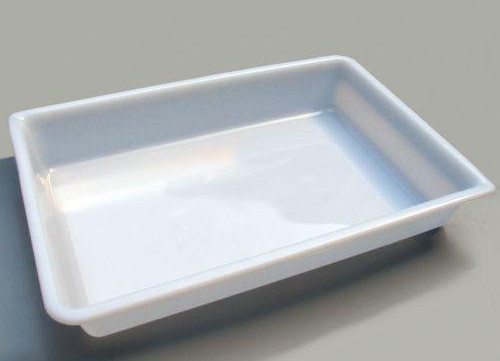
\includegraphics[width=0.4\textwidth]{capitulo-5/graphics/bandeja-muestra.jpg}} &
        \num\putindeepbox[7pt]{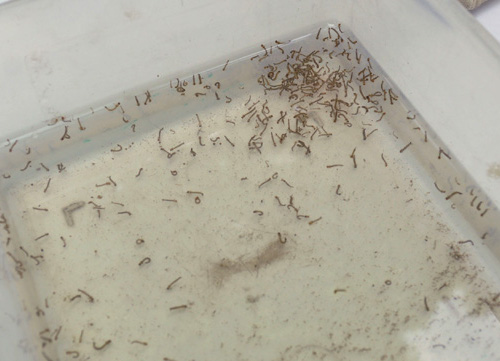
\includegraphics[width=0.4\textwidth]{capitulo-5/graphics/larvas-dengue.jpg}} \\
    \end{tabular}

    \caption{\label{fig:cap5-conteo-pdi-bandejas} Bandejas de plastico utilizadas como contenedor
    de larvas.}

    \footnotetext[1]{Bandeja de muestra vacia, sin larvas.}
    \footnotetext[2]{Bandeja con larvas correspondientes al un punto de control.}
\end{minipage}
\end{figure}

Exiten diferentes métodos para el análisis de imágenes que nos permiten realizar el conteo de
larvas teniendo en cuenta las caracteristicas de las larvas. Presentaremos el método y las técnicas
utilizadas para la realizar el conteo de forma tivial, pero dista mucho de ser trivial y un
análisis más profundo escapa al alcance de este proyecto.

El método seleccionado para realizar el conteo fue el de Otsu, ya que no requiere supervición
humana ni información previa de la imágen antes de su procesamiento. Este método se emplea cuando
hay una clara diferencia entre los objetos a extraer respecto del fondo de la escena
\citep{santillan2008deteccion}. Con la finalidad reslatar las caracteristicas de las larvas,
estas deben depositarse en una bandeja de plástico de color blanco para posteriormente realizar la
captura.Como se puede apreciar en la \figref{fig:cap5-conteo-pdi-bandejas}, con esto se consigue
un contraste entre el fondo las larvas observadas.

La imagen se transforma a escala de grises, se ajusta el histograma para mejorar su contraste y se
calcula su umbral mediante el método de Otsu (\figref{fig:cap5-larvas-otsu}).

\begin{figure}
\begin{minipage}{\textwidth}
    \begin{tabular}{c c }
        \initbox
        \num\putindeepbox[7pt]{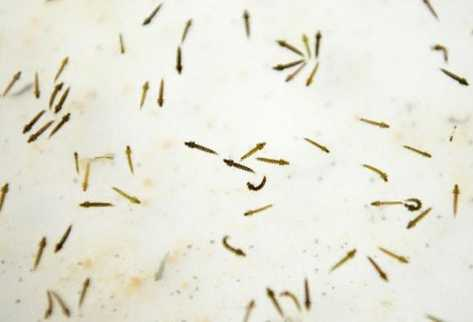
\includegraphics[width=0.4\textwidth]{capitulo-5/graphics/larvas-original.png}} &
        \num\putindeepbox[7pt]{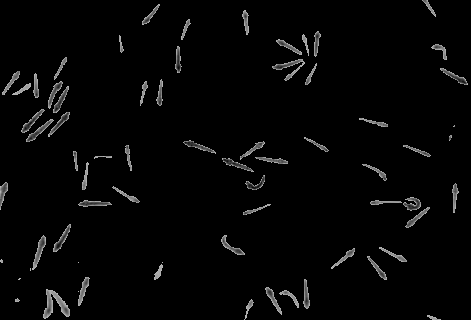
\includegraphics[width=0.4\textwidth]{capitulo-5/graphics/larvas-otsu.png}} \\
    \end{tabular}

    \caption{\label{fig:cap5-larvas-otsu} Transformación de la una imágen mediante el método de
    Otsu.}

    \footnotetext[1]{Imágen original.}
    \footnotetext[2]{Imágen luego de la umbralización de Otsu.}
\end{minipage}
\end{figure}

Se definen 2 conjuntos, el primero corresponde a los objetos dentro de la imagen, las larvas, y el
segundo al el fondo, recipiente con el agua que contiene las larvas. Luego definimos el umbral $T$
que determina si un píxel pertenece a un grupo u otro según su nivel de gris $g$. La función $f$
torna 1 o 0 por cada píxel.

\begin{equation}
\label{eq:umbralizacion-otsu}
f(x, y) =\left\{
  \begin{array}{l l}
    1 & \quad g > T\\
    0 & \quad g \leq T
  \end{array} \right.
\end{equation}

Como se observa en la ecuación \eqref{eq:umbralizacion-otsu}, se analiza simplemente el nivel de
gris correspondiente a cada píxel y se determina si forma parte de un objeto de estudio o si forma
parte del fondo.
